\def\year{2015}
\documentclass[letterpaper]{article}
\usepackage{aaai}
\usepackage{times}
\usepackage{helvet}
\usepackage{courier}

\usepackage{listings}
\usepackage{color}
\usepackage{xspace}
\usepackage{graphicx}

\newcommand{\ceg}[1]{{\textcolor{blue}{#1 -- CEG}}}
\newcommand{\cpg}[1]{{\textcolor{red}{#1 -- CPG}}}
\newcommand{\eat}[1]{}
\newcommand{\system}{\textsl{Grisham}\xspace}

\frenchspacing
\setlength{\pdfpagewidth}{8.5in}
\setlength{\pdfpageheight}{11in}
\pdfinfo{%
/Title (A Topic-Based Search, Visualization, and Exploration System)
/Author (Christan Grant, Clint P. George, Virupaksha Kanjilal, Supriya Nirkhiwale, Joseph N. Wilson, Daisy Zhe Wang)
/Keywords (Topic Modeling, Latent Dirichlet Allocation, Topic Search, User Model, Exploration)
}

\setcounter{secnumdepth}{1}  

\begin{document}

\title{A Topic-Based Search, Visualization, and Exploration System}
\author{Christan Grant, Clint P. George, Virupaksha Kanjilal, Supriya Nirkhiwale, \\ 
{\bf \Large Joseph N. Wilson, Daisy Zhe Wang}\\
Computer and Information Science and Engineering, University of Florida}

\maketitle


\begin{abstract}

From literature surveys to legal document collections, people need to organize and explore large amounts of documents.
During these tasks, students and researchers will search for documents based on particular themes.
In this paper, we use a popular topic modeling algorithm, Latent Dirichlet Allocation, to derive topic distributions for articles.
We allow users to specify personal topic distribution to contextualize the exploration experience.
We introduce three types of exploration: \textsl{user model re-weighted keyword search},
\textsl{topic-based search}, and \textsl{topic-based exploration}. 
We demonstrate these methods using a scientific citation 
data set and a Wikipedia article collection.
We also describe the user interaction model.

\end{abstract}



\section{Introduction}

In a variety of situations, from literature surveys to legal 
document collections, people try to organize and explore large 
amounts of documents. Current technology to search on documents are 
done based on keywords with minor extensions. Keyword-based search is useful when the 
user knows exactly what he or she is looking for. It is not 
particularly useful when a user wants to explore or learn a new 
topic. 
The difficulty with keyword-based search is especially pronounced when, for
example, a researcher wants to find out the state of the art in a particular
area or a student would like to create a literature survey. In such situations,
\textsl{topic-based search} can return more relevant results. 
Topic-based search is a classification of the search space to 
highlight topical relevance. In order to accomplish this, the topics 
underly documents across collections need to be extracted, and then 
the documents have to be represented in terms of those topics and ranked 
based on relevance to a particular topic. 

In our system called \system we present various techniques for topic-based exploration 
and search of articles. Our work allows users 
to search for documents using three paradigms. 
First, users may perform a traditional keyword-based search for papers.
The results are re-ranked based on a topic distribution specified by the user. 
Second, user may perform a \textsl{topic-based search} where the user specifies 
a topic she is interested in and documents will be returned ordered by their relevancy to the topic.
Lastly, users may explore topically similar documents using a visual 
graph like interface.


\eat{The main contributions of our work are the \textit{user-topic ranking function} 
which ranks the relevance of documents to a set of topics---\cpg{I 
think we need to edit this; a similar ranking function is there in 
\citeauthor{George2012}~\citeyear{George2012}}, the 
\textit{similar document explorations} which is performed by computing the 
similarity of papers to a topic of interest, and \textit{topic-document visualization} which 
ranks citations for a paper by the interest of the user.
}

This paper discussed the implementation of three search and exploration paradigm that are a developed inside of \system.
The main contributions of this work are as follows:
\begin{itemize}
\item A search based on user-defined preferences.
A user can interactively define a topic-based model for their search preferences.
\item An implementation of ranking functions for topic-based search.
\item A novel interaction model for topic-based exploration.
\end{itemize}

This paper is organized as follows.
In Section~\ref{sec:topicmodels}, we give an introduction to topic models.
In Section~\ref{sec:system}, we describe the theoretical structure of \system.
In Section~\ref{sec:demo}, we describe the user interface and the user interaction model.
Finally, we conclude this paper with a discussion of related work in Sections~\ref{sec:discussion} and~\ref{sec:summary}.




\section{Topic Models}
\label{sec:topicmodels}

Topic models are a set of models for the documents in a collection 
or corpus. They enable us to represent properties of a large 
corpus containing numerous words with a small set of \textsl{topics}, 
by extracting the underlying topical structure of the corpus and 
representing the documents according to these topics. We can then 
use these representations for organizing, summarizing, and searching 
the corpus. Traditionally, topic models assume each word occurrence 
within a document is independent. This is the assumption of ``bag of 
words'' models. Latent Dirichlet Allocation or LDA 
\cite{Blei2003} is a well known, generative, probabilistic   
topic model for a corpus. A probabilistic generative model assumes 
data as \textsl{observations} that originate from a generative 
probabilistic process that includes \textsl{hidden} variables. The 
hidden variable are typically inferred via \textsl{posterior 
inference}. In posterior inference, one tries to identify the posterior 
distribution of the hidden variables that are conditioned on the observations. 
Loosely speaking, one can consider posterior inference as the 
reverse of the generative process. LDA assumes 
that there exists a set of \textsl{latent} (hidden) topics for a 
give corpus. A topic is defined as a distribution over the corpus 
vocabulary. The topics are assumed to be generated from a 
\textsl{Dirichlet} distribution with a set of parameters. For 
example, a topic about \textit{whales} will have words related to 
whales and related topics (e.g., \textit{blue whales}, \textit{killer whales}, 
\textit{whaling}, etc.) with high probability and words related to 
other unrelated topics (e.g., \textit{sports}, \textit{medicine}, 
etc.) with low probability---assuming the corpus is built from a 
subset of articles from the topics \textit{whales}, \textit{sports}, and 
\textit{medicine}. In addition, each document in the corpus is 
described by a latent topic distribution and the words in a document 
are generated from the document specific topic distribution. The 
document topic distributions 
are also assumed to be generated from another \textsl{Dirichlet} 
distribution with a set of parameters. In real life, we only observe 
documents and their words. As in any generative probabilistic model, 
the latent variables in the LDA model are typically identified by 
posterior inference. 

Unfortunately, in most of these generative models, posterior 
inference is intractable due to the high dimensionality of the 
latent variable space, and practitioners typically rely on 
approximate posterior inference alternatives. For the LDA model, 
people have used different approximate inference methods such as 
deterministic \textsl{optimization methods}~\cite{Blei2003} and 
\textsl{sampling methods}~\cite{Griffiths2004} for the inference. 
\citeauthor{Blei2003} employed variational methods to find 
approximations to the posterior distribution of latent variables, by 
posing a family of lower bounds on the log likelihood indexed 
by a set of variational parameters. The variational parameters are 
then identified by a deterministic optimization procedure that seeks 
to find an optimal lower bound. \citeauthor{Griffiths2004}'s method 
was based on Gibbs sampling---a Markov chain Monte Carlo 
method that helps to approximate the intractable posterior integral 
as an empirical estimate of the samples generated from a Markov chain.   
In Gibbs sampling, one forms the Markov chain by repeatedly sampling 
each variable conditional on the most recently sampled values of the 
other variables~\cite{Geman1984}. In this paper, we use the scalable 
implementation of the online variational inference algorithm for LDA
\cite{hoffman2010online} by~\citeauthor{rehurek_lrec} 
\citeyear{rehurek_lrec}. 


Due to the fully generative semantics, even at the level of 
documents, LDA is expected to overcome several drawbacks such as 
synonymy and polysemy of words where in earlier models, e.g., TF-IDF
\cite{Salton1975} and Latent Semantic Analysis (LSA, \citeauthor{Dumais1995} 
\citeyear{Dumais1995}). In this paper, we are interested in the LDA 
model parameters such as the corpus-level latent topic distributions 
and document-level latent topic distributions. The latent document 
topic distributions are lower dimensional representations of 
documents (which traditionally are vocabulary-size term-frequency vectors) 
and useful for finding and grouping similar documents in a corpus. 
The latent topics in a corpus, which are distributions over the 
vocabulary terms, are helpful in visualizing the prevalent thematic 
structure of a corpus and exploring documents related to a specific 
theme of interest. In the \system section, we describe how we 
exploit these model parameters.   

Now we describe the notation we use in this paper. For a given corpus, 
let $D$ be the number of documents in the corpus and $V$ be the 
number of terms in the corpus vocabulary. The number of topics $K$ 
in the corpus is a constant and known. For $d = 1, 2, \ldots, D$, we 
denote the $K$ dimensional vector $\theta_d^{*}$ as the estimate of 
document $d$'s latent distribution on the topics identified via an 
approximate posterior inference algorithm. In addition, for $j = 1, 
2, \ldots, K$, we denote the $V$ dimensional vector $\beta_j^{*}$ as 
the estimate of $j$th topic distribution. This forms a $K \times V$ 
topic matrix, whose $j$th row is the $j$th topic and each element 
$\beta_{jt}^{*}$ represents term $t$'s probability for the 
$j$th topic.   




\section{\system}
\label{sec:system}


{\system} system is built to process articles,
provide fast response to user queries and display descriptive
results in a user interface.
In this section we describe our pre-processing steps to extract
topic models from the documents.
We then discuss the \textsl{user model} behind each user search and 
\textsl{user model} re-weighted keyword search.
Finally, we discuss our methods for topic-based search and exploration.



\subsection{Data pre-processing and topic learning}

Here we describe the main pre-processing steps we perform on a 
collection of articles for topic modeling and search. First, 
we tokenize articles with the help of the python 
Natural Language Toolkit (NLTK)~\footnote{\texttt{http://www.nltk.org/}} and a set of 
predefined regular expressions. Next, we standardize tokens by 
removing noise and stop-words. We use typical normalization 
techniques for word tokens such as \textsl{stemming}, in particular we use the popular Porter stemming algorithm~\cite{Porter1980} 
implementation in NLTK\@. 
After building a vocabulary of corpus words, each document is represented as a sparse ``bag of words''.
Last, we use the processed documents as input to the topic 
learning algorithm~\cite{hoffman2010online} which will in turn learn 
the latent topic structure of a corpus from the term co-occurrence 
frequencies of the corresponding documents. 



\subsection{User Model}
When performing search, exploration and discovery over articles 
users may bring particular context to their search. Incorporating 
this information into the search process has been shown to be 
beneficial to users~\cite{DZSRWJ,MZPGSOL}. We develop a user model 
that encapsulates the users personal context and integrates it into 
their search task. 

This model is a distribution of weights for each identified topic in 
a corpus. Formally, given a set of topics $\beta_j^{*}$s the user 
model is defined as
$$
\mathcal{U} = \{u_0, \ldots, u_{K}\}
$$
where $u_j \in [0,1]$, $\sum_{j = 1}^K u_j = 1$, $K$ is the number 
of topics in the corpus.
We allow the user to interactively select the weights that correspond to
each topic learned over the corpus. This allows the users to change preferences with each query
for more desirable results.

\subsection{User Model Re-weighted Keyword Search}
The user model is used to provide better feedback to
the user. After a \textsl{keyword-based filter}, the document results of the search 
are re-ranked using the KL-divergence of each document and the
user model. Formally, given the set of result documents $\cal D$:

\begin{equation} \label{eq:KL}
KL(\mathcal{U}||\theta^*_{d}) = \sum_{j = 1}^K u_j \ln \frac{u_j}{\theta^*_{dj}}.
\end{equation}
where $d \in {\cal D}$ and $\theta^*_{d}$ is the topic proportion 
for document $d$ from the LDA model. 


\subsection{Topic-Based Search}

Another method of search is to identify the topics of 
real interest, observing the most \textsl{informative terms} in 
the estimated topics. 
To identify informative terms in a topic we can sort vocabulary 
terms in the order of their term probabilities.
That is, each vector $\beta_j^{*}$ in the topic matrix is sorted.
  
In literature, researchers have proposed several other methods for 
finding informative terms~\cite{2012-termite} and evaluating topics 
\cite{mimno2011optimizing}. In this paper, we use a visualization 
scheme called \textsl{word cloud}~\cite{Davis2013}, to visualize the 
most probable words in a topic. For example, see Figure 
\ref{fig:topic-word-cloud} for the visualization of a topic that is 
extracted from a corpus, which is built from a subset of Wikipedia 
articles under the category \textsl{Whales}. 
       
\begin{figure*}[htb]\centering 
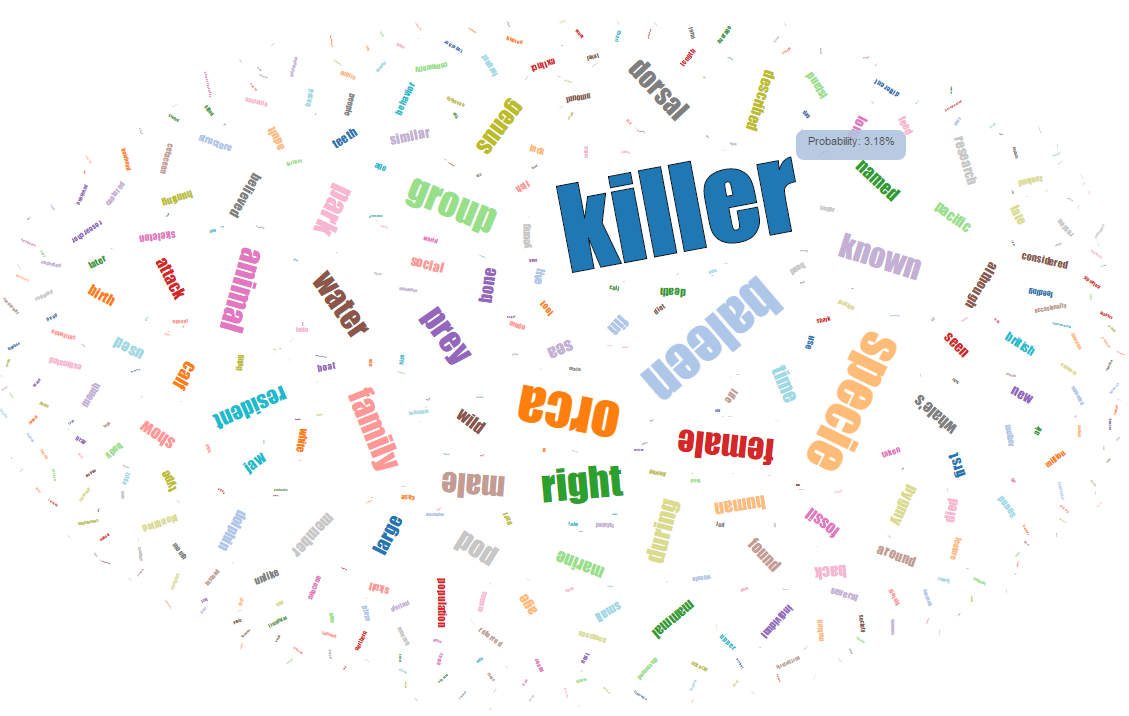
\includegraphics[width=.8\textwidth]{topic_visualization.png}
\caption{\textsl{Topic Word Cloud}. Words with high probabilities for the 
given topic are larger in size and words with low probabilities for 
the given topic are smaller in size. From the most probable words, 
we can infer that the topic mainly refers to the Wikipedia category 
\textit{Killer Whales}---one of the main categories from which, we 
downloaded the articles for the corpus.}
\label{fig:topic-word-cloud}
\end{figure*}

We can exploit the estimated document specific topic distributions 
 of individual articles ($\theta_d^{*}$) in a corpus, to rank them on 
relevance for given a topic. Let $t$ be the index for the topic of 
interest. For each document $d = 1, 2, \ldots, D$ in the corpus, we 
can calculate~\cite{George2012}
\begin{equation}
m(d) = \ln \theta^*_{dt} + \sum_{j \neq t}{\ln (1 - \theta^*_{dj})},
\label{eq:topic-exploration}
\end{equation} 
where $j = 1, 2, \ldots, K$ and each $\theta^*_{dt}$ is 
normalized, i.e., $\sum_{j=1}^{K}{\theta^*_{dj}} = 1$. We then sort 
the documents based on each $m(d)$ to rank them on relevance. 
Intuitively, we can see that Equation~\ref{eq:topic-exploration} 
will give a high value for a document, if the document is 
thematically related to the $t$th topic. 

\subsection{Topic-Based Exploration}

If a user find an interesting document and she would like to
find other similar documents she may use the topic-based method of exploration.
To visualize the hidden topical content of the article we use the 
estimated document topic distribution, $\theta^*_{d}$.
For example, Figure~\ref{fig:doc-topic-distribution} shows a Doughnut  
Chart\footnote{\texttt{https://developers.google.com/chart}} 
visualization for the Wikipedia article \textit{Killer Whale}.
It is an article listed under the Wikipedia category          
\textit{Killer Whales}. Different slices of the doughnut chart represent
different topics in the article \textit{Killer Whale}. The size 
of a slice represents the probability of a topic given the article. 
For this illustration, we labeled all the topic 
distributions obtained via the LDA posterior inference, on a 
corpus that is built using a subset of Wikipedia articles under the 
category \textit{Whales}. We used the topic word clouds 
and the Wikipedia subcategories under the category \textit{Whales} 
for labeling. Once we find an interesting topic to pursue, we can 
explore all the relevant documents under that topic using the 
method described in the previous section. 

\begin{figure}[htb]\centering 
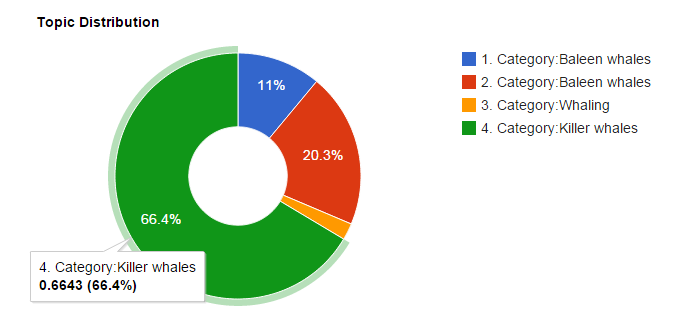
\includegraphics[width=.45\textwidth]{doc_topic_distribution.png}
\caption{Visualization of the document specific topic distribution 
for the Wikipedia article \textit{Killer Whale}.}
\label{fig:doc-topic-distribution}
\end{figure}

Another way to visualize a document is to look at its 
\textsl{paragraph} or \textsl{section} specific topic distributions. 
Each section or paragraph is written with careful attention in every 
peer review article or paper. While looking at an article or paper,  
one can easily identify which section or paragraph is of one's real 
interest. This intuition can be used to improve topic based 
exploration. We used the learned LDA model to 
estimate a section or paragraph's topic distribution using the
Gensim LDA implementation~\cite{rehurek_lrec}. This is an 
online task and is performed when a user selects a section or 
paragraph of an article, which is described in detail in the \system 
User Interface section.


Another interesting option to explore is how we can use an article's 
topic distribution for searching similar articles of interest. 
Recall that LDA enables us to transform documents in a corpus into 
vectors ($\theta^*_{d}$) in a lower dimensional topic space 
of that corpus. One can then define similarity between two documents 
via any typical vector space similarities, e.g., cosine similarity. 





\section{User Interface}
\label{sec:demo}


To demonstrate \system's exploratory search we loaded scientific 
papers from the DBLP conference~\cite{Tang:2008:EMA:1367497.1367722} 
and also Wikipedia articles downloaded using the MediaWiki API~\footnote{\texttt{https://www.mediawiki.org}}.
The {\system} website has a list of topics with a slider associated 
with each of them using which a user can specify the degree of 
interest in that particular topic. The weightage specified by each 
slider corresponds to the components of the user model. The user 
model is a profile of preference provided by the user before she 
makes any search.

Initially, all the extracted topics from the corpus are shown along 
with their most informative words (see Figure~\ref{fig:topic_exploration}).
This list is color coded to distinguish the relevance of topics as indicated by the user model --- much like a heat map.
The user can look at this heat map to adjust their topic preferences.
The list is clickable and once a topic is selected, relevant articles to that topic ranked based on the user model are displayed.
In the \textsl{Graph Explorer} interface, the citations for the current article is ranked
using Equation~\ref{eq:KL}. The citations (of that article) that are most
similar to the user model are ranked the highest.



The tab \textsl{Keyword Paper Search} (Figure~\ref{fig:topic_exploration}) contains the interface for the user model weighted keyword search.
The user may enter one or more keywords representing topics,  
author names, etc. The keywords are searched in the title, abstract, 
and author fields of all the articles. The discovered results are  
re-weighted using the user model. 
\eat{
In the first page only a few of 
the articles are displayed in two boxes --- one containing matching words in the title, and the other in the abstract.
Clicking on any box will open up a more complete list of articles.}

\begin{figure}[htb]\centering
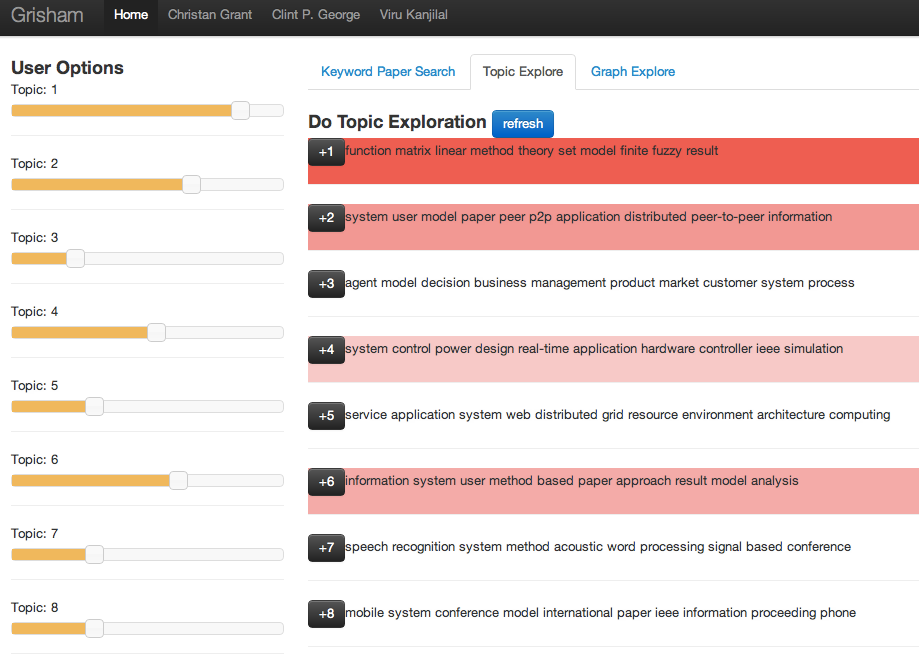
\includegraphics[width=.45\textwidth]{topic_exploration.png} % scale=.25,trim=0 0 300 0
\caption{The interface for examining the effect of changes to the user model on the topics.}
\label{fig:topic_exploration}
\end{figure}

For topic exploration \system allows a user to click on a specific 
topic to see the informative words for that topic in a word cloud 
(Figure~\ref{fig:topic-word-cloud}). By selecting a topic the user 
can explore more about the articles associated with the topic using 
Force-Directed Graph~\cite{2011-d3} (Figure~\ref{fig:topic-search-viz}).
A user can navigate to a particular document by clicking a document 
node (orange) in the graph. 

On the document visualization page, we show a doughnut chart for the document topic distribution as well as a preview of the document contents.
Clicking on the topics in the doughnut chart will take the user to the topic word cloud page.
Selecting a section or paragraph changes the doughnut chart to reflect the topic distribution specific to that selection.
For example, the document visualization page for \textit{Killer whale} is displayed in Figure~\ref{fig:doc-para-viz}.





\begin{figure}[htb]\centering 
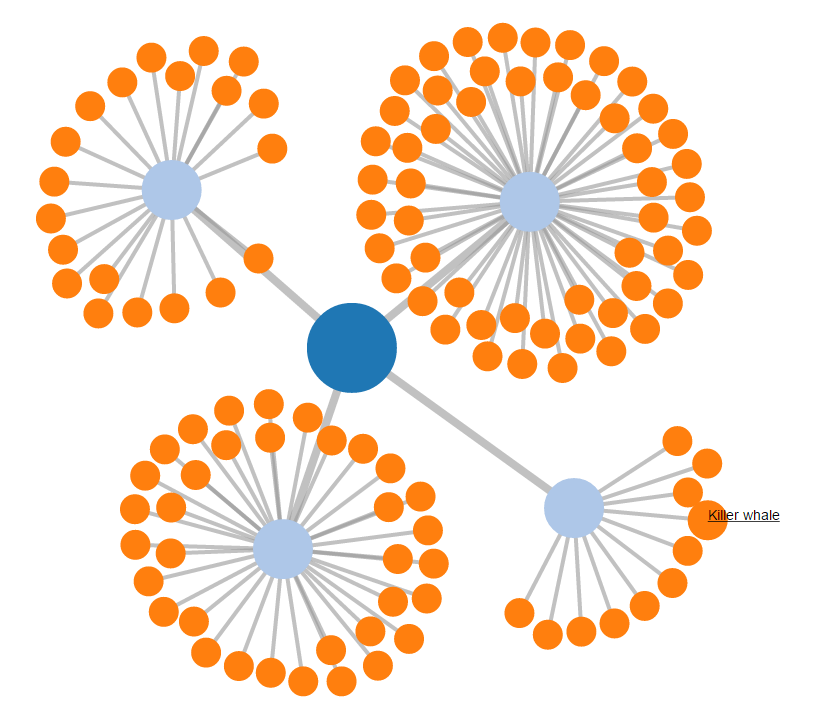
\includegraphics[width=.5\textwidth]{topical_docs.png}
\caption{Visualizing \textsl{topic-based search} in \system, orange 
nodes represent documents and blue nodes represent the estimated 
topics in a corpus. For this illustration we only show four topics 
(light blue nodes). Topic names appear when the user hovers over a 
node.}
\label{fig:topic-search-viz}
\end{figure}

\begin{figure*}[htb]\centering 
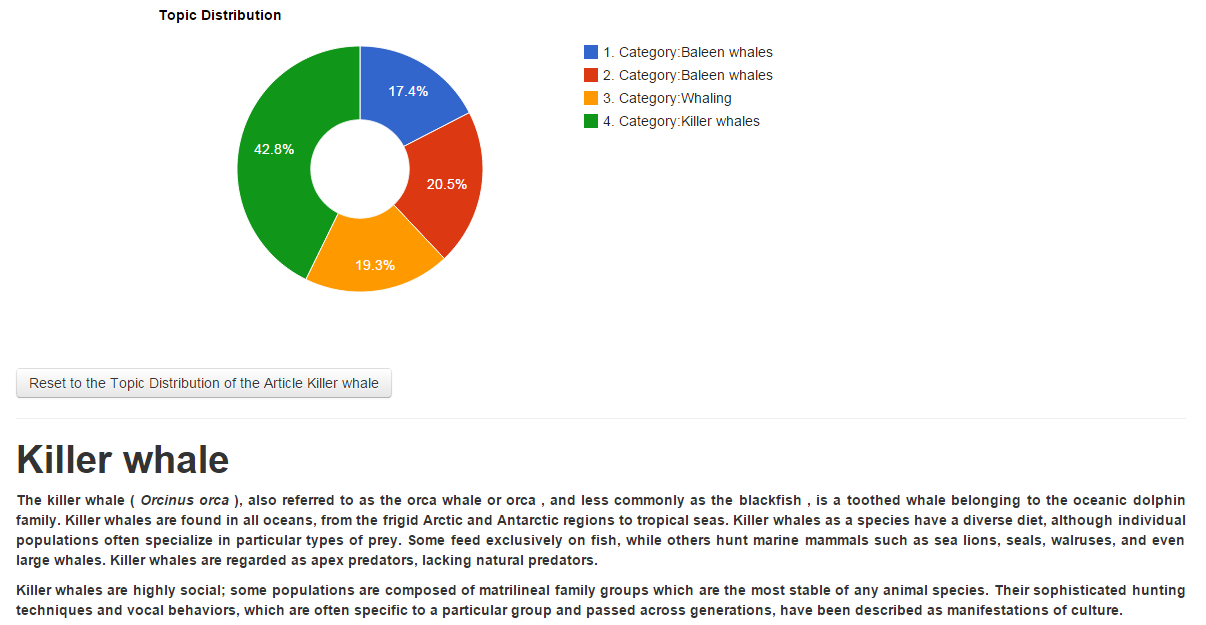
\includegraphics[width=1\textwidth]{para_topic_distribution.png}
\caption{Visualizing the topic distribution of the introduction 
section of the Wikipedia article \textit{Killer Whale}. See Figure~\ref{fig:doc-topic-distribution} for the topic distribution of 
the whole article.}
\label{fig:doc-para-viz}
\end{figure*}

\eat{
\begin{figure}[htb]\centering 
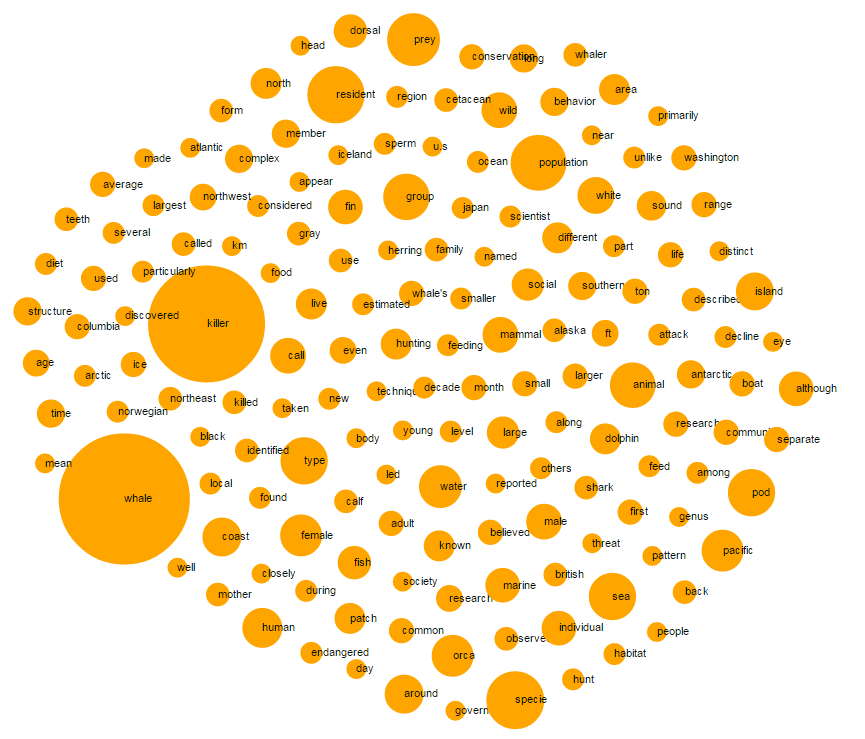
\includegraphics[width=.5\textwidth]{doc_tf_bubble_chart.png}
\caption{Visualizing the relative frequencies of terms in the 
Wikipedia article \textit{Killer Whale}. \cpg{I think we need to 
decide whether we should keep this figure in the paper or not.}}
\label{fig:doc-word-counts}
\end{figure}
}


The \textsl{Graph Explore} interface allows a user to recursively 
drill down a graph of an article and its out-links (citations).
This is a common method of literature exploration; a user takes up a base article and then reads all the articles which have been cited in that base article.
These steps are recursively performed for each subsequent article until the user has found a sufficient amount of articles or they have read all the articles in their collection.
The graph explore interface allows a user to perform this in a more visually appealing manner.
Once a user decides on a base article (through any search scheme), the system shows a graph representation of its citations which are ranked based on her profile (i.e. \textsl{user model}).
This will help her pursue the most relevant articles first.
Clicking on any secondary article will expand the graph further and 
list secondary citations ranked based on the \textsl{user model}.




\section{Discussion and Related Work}
\label{sec:discussion}

A system of note is Yang et al.~\cite{yang2011topic} who applied topic modeling to 
collections of historical news papers to assist search. They 
found that the topics generated from topic models are 
are generally good, however once the sets of topics are 
generated, an expert opinion is required to name them. 
In \system, we allow users to select numbered topics for article-search 
based on topically relevant words.


Termite~\cite{2012-termite} provides a visual analytic tool for assessing topic
quality that allows for comparison of terms within and across latent topics.
They introduce a saliency measure that enables the selection of relevant terms.
For a particular topic, the system provides the word frequency distribution
relative to the full corpus and shows the most representative terms according
to the saliency measure.

A number of previous
work~\cite{chang2009reading,mimno2011optimizing,newman2010evaluating} depended
heavily on experts examining lists of the most probable words in the topic and
validating the models. Hall et al.~\cite{hall2008studying} applied unsupervised
topic modeling to study historical trends in computational linguistics across
14,000 publications. The work required experts  to validate the quality of the
results. Only 36 out of 100 topics were retained, and there were 10 additional
topics that were not produced by the model and had to be manually inserted.


For visualizing the results, previous work~\cite{2012-termite,bertin1983semiology,henry2007matlink} use
 a matrix style view to surface the relationships between many terms. 
These tools are created for evaluating topic models.
Interacting with such visualizations can be complex because the user should
already have an intuition about the results in advance in order to properly generate necessary
orderings.
Leake et al.~\cite{leake2003topic} provide methods to aid concept mapping by suggesting relevant information in the context of topics models, represented as concept maps. 

Wu et al. have created an advanced full-text search engine for academic articles~\cite{wu2014citeseerx}.
This project can be viewed as the state of the art in this area.
However, we have not found any evidence that they integrate topic modeling techniques to further search.
Integration of the user model with the CiteSeerX system is an interesting research direction.




\section{Summary}
\label{sec:summary}

We describe \system, a system for topic-based article search
and exploration given a user model.
This paper describes a promising search paradigm.
Any researcher who would like to do exploratory search or literature 
reviews will find the system beneficial. In the future, 
we would like to perform user studies to obtain feedback on the 
effectiveness of the three search paradigms.


\section{Acknowledgements}

This material is based upon work supported by the NSF Graduate 
Research Fellowship under Grant No. 
DGE-$0802270$ and the International Center for Automated 
Research (ICAIR) at the UF Levin College of Law. 
This work was also supported by a generous grant from DARPA under
FA8750-12-2-0348-2 (DEFT/CUBISM).


\bibliography{citation}
\bibliographystyle{aaai}

\end{document}
